
\section{Introduction}

At DASIA 2017\cite{Lero-DASIA17}
we discussed a modular approach to formally modelling
requirements, using a requirements baseline for a separation kernel developed
as part of the IMAKQP project\cite{IMAKQP-D02}.
This was based on work done using the CSP formalism\cite{hoare-1985:commuseque:},
done by two students for their dissertations \cite{KH-MCS2016,Costelloe17}.
Properties of interest could be explored and verified using
model-checking software such as FDR \cite{FDR3}.
That work followed on from recommendations we made for future work
in this area, including:
formalising the requirements baseline;
formalising kernel data-structure invariants;
and completing rough/draft CSP models explored during IMAKQP.

We consider that many useful formal modelling paradigms in this space
fall into two broad classes:
\begin{description}
  \item [State-Based]
    These are based on the notion of mutable state,
    usually organised as named variables, updated by assignment.
  \item [Process-Based]
    These communicate by message-passing, and persistent state
    is modelled as parameters to a process description.
    State change is captured by invoking the process with revised parameter values.
\end{description}
We shall illustrate these two paradigm classes by modelling a simple counter
system that supports two operations: counter initialisation, and count-up,
The count is observable, somehow.

\subsection{State-based Modelling}

A classic example of the state-based paradigm is
the Z specification language \cite{UsingZ}.
Here we consider the counter state as being stored
in a variable called $count$. Initialisation sets this variable to zero,
while counting up or down result respectively
in the variable being incremented or decremented.

In Z, which is a \emph{specification} language,
we model operations as relating their starting state (variable values)
to acceptable final states. Given variable \texttt{v},
we use the mathematical/logical variable $v$ to denote its starting value
before the operation commences,
and $v'$ to denote its value once the operation has completed.
In Z, a box-like graphical notation is used that has an operation name,
along with a declaration of its state observation variables,
follwed by predicates that describe the desired relationships that should hold.
\begin{schema}{CountInit}
  count,count' : \num
\where
  count' = 0
\end{schema}
\begin{schema}{CountUp}
  count,count' : \num
\where
  count' = count+1
\end{schema}
Z is very much aimed at specifying in a way
that suits ``standard'' imperative programming styles.

\subsection{Process/Event-based Modelling}

In the CSP formalism, we have (parameterised) processes
that participate in ``events'', and who subsequent behaviour
can depend on which event has just occurred.
We will imagine two events "init" and "up" that model respectively
the invocation of initialisation or counting-up.
We have a process called $Count$ that
is paramterised with a value we call $count$.
It's behaviour is that it performs
an ``external choice'' operation ($\extchoice$)
in which it offers to participate in either of the $init$ or $up$ events,
and then invokes itself recursively with a suitable revised parameter.
\begin{circus}
\circchannel init, up \\
Count(count) \circdef \\
\t1 init \then Circus(0) \\
\t1 \extchoice \\
\t1 up \then Count(count+1)
\end{circus}
The focus in CSP is on inter-process communication and concurrency.
This makes it very suitable for modelling requirements in a compositional
way, and is why it was initally chosen
as  a basis for modelling the IMAKQP baseline.
However, one problem with this approach is that the number of parameters
per process can get very large,
and state-changes that modify these are hard to scan and digest.

\section{Unification}

The work reported here explores a technique that aims to have the best of both
worlds, based on a formal paradigm known
as ``Unifying Theories of Programming'' (UTP) \cite{UTP-book}.
This uses 2nd-order classical predicate calculus,
where every predicate has an ``alphabet'' of variables that
model observations of a system that it is capable of describing.
The predicates relate before- and after-observations of a system,
using a similar convention that found in Z.

We do not go into details here, but show some standard UTP definitions
to give a flavour for how it works:

\begin{tabular}{ll}
\hline
   \textbf{Command} & \textbf{Semantics}
\\\hline
     $x:=e$
   & $x'=e \land v'=v$
\\   $P~;Q$
   & $\exists v_0 \bullet P[v_0/v'] \land Q [v_0/v]$
\\   $P\sqcap Q$
   & $P\lor Q$
\\   $P \lhd b \rhd Q$
   & $b \land P \lor \lnot b \land Q$
\\   $P \sqsubseteq Q$
   & $[Q \implies P]$
\\\hline
\end{tabular}

Simple examples of unification include our ability to immediately define
standard verification methodologies such as
Hoare Triples (HT)
and Weakest Precondition (WP), in terms of standard definitions:
\begin{eqnarray*}
   \{p\} Q \{r\} &\defs& (p \implies r') \sqsubseteq Q \qquad (HT)
\\ Q ~\textbf{\textsf{wp}}~ r       &\defs& \lnot (Q ~;\lnot r) \qquad (WP)
\end{eqnarray*}


\subsection{State-rich Processes}

An alternative approach to just using Z, or CSP,
is taken by the language \Circus\cite{WC01,OCW2007},
which is a fusion of CSP with Z.
This allows individual named state components to be modified using simple
assignment statements, making descriptions easier to read.
It's formal semantics has been defined using UTP\cite{OCW2007}.
For example, our counter might be generated as follows:

\begin{circus}
\circchannel init,up \\
\circprocess Counter \defs \circbegin \\
\circstate State \defs [count:\num] \\
\t1 Count \defs \\
\t2 init \then count := 0 \\
\t2 \extchoice \\
\t2 up \then count := count+1 \\
\t1 Run \defs Count~; Run \\
{} \bullet count := 0 ~; Run \\
\circend
\end{circus}

We have operations being invoked using the $init$ and $up$ events
as for the CSP example, but we also have a state containing a variable $count$,
which is modified by using assignment.


The \Circus\ language has been used to model requirements
for a haemodialysis machine\cite{DBLP:conf/asm/GomesB16},
in a similar way to how CSP was used to model kernel requirements.
This exploits the ability of \Circus\ to focus only on the relevant state changes.

\subsection{Translation}

There is a state-of-the-art model checker for CSP, called FDR
(``Failures-Divergences Refinement'') \cite{FDR3}.
However, as there is, as yet,no model-checker for \Circus,
the standard approach in the literature is to carefully translate
a \Circus\ model into a CSP one, to make use of FDR.
We did this with our haemodialysis model\cite{DBLP:conf/asm/GomesB16},
but orberved that it was a very error-prone process.
This lead us to develop an automated semantics-preserving
translator from \Circus\ to CSP
that allows FDR to be used for analysis.

This translation is based on one developed in the EU-funded FP7 COMPASS project,
and is described in Deliverable D24.1 of that project\cite{compassd241}.
It gives a formal specification of rules to follow when
translating  Circus to CSP by hand.
Some of these rules have been verified using manual proof,
and some with the Proofpower Z theorem-prover\cite{PPZRM}.
The main idea behind this translation is that
all the explicit (mutable) \Circus\ variables are collected as parameters
of a CSP memory process, that accepts $get$ and $set$ events
for each variable. The assignments in the \Circus\ part
are then replaced by appropriate invocations of these events,
resulting in what is in effect a pure CSP process.
The system becomes the memory process running in parallel with the
assignment-free CSP process.
The mutable variable state has become a large parameter of the memory process.

We  implemented this in Haskell,
following the translation scheme as defined in \cite{compassd241},
with some additional optimisations.
The optimisations addressed some issues with the CSP type-system,
and resulted in the big monolithic memory process being broken
into a collection of smaller independent memory processes.
Initialy forced on us as a result of typing issues,
we noticed considerable improvement of the model-checking
each time we split the memory process.
We have ended up with a translation were each original \Circus\ variable.
To illustrate this improvement,
consider the following results,
obtained by doing a deadlock-freedom check on a model of a haemodialysis
machine, in which certain variables were notional of type $\num$.
Because model-checkers need finite models to work at all,
we needed to decide what range of values $\num$ would actually have.
Here ``byHand'' denotes the original D24.1 translation scheme,
while ``CTOC'' is the fully optimised version

\begin{tabular}{|c|c|c|c|}
\hline
   Approach & $\num$ & Outcome & Time (sec.)
\\\hline\hline
          & 0\dots1 & Passed & 40.8
\\\hline
  byHand  & 0\dots2 & incomplete & $>$ 2 hours
\\\hline\hline
          & 0\dots1 & Passed & 0.375
\\\hline
          & 0\dots2 & Passed & 0.407
\\\hline
  CTOC    & 0\dots10 & Passed & 0.937
\\\hline
          & 0\dots90 & Passed & 35.1
\\\hline
\end{tabular}

We see that with the byHand version we can only check a version
with $\num = \{0,1\}$,\
but the CTOC translation can handle $\num=\{0,\dots,90\}$
in less time!


\section{Requirements Modelling}

An event is an abstraction of an observation of some change
or communication in a system. Events are considered atomic
(they happen completely, or not at all), and instantaneous.
An event can also have internal structure,
so it can be used to carry information over and beyond
just signalling that it has occurred.
The behaviour of a system is defined in terms of:
(i) all the possible sequences of events that can be observed;
(ii) at each stage, what events are being blocked.
The state of a system captures which events it is willing to perform,
along with information about how its future behaviour depends on those events.
State can be represented implicitly by the ``call-graph'' structure of the model,
or, additionally,
some parts are given explicity as components whose values can change.

Typically, we build models with three key components,
each of which runs in parallel with the others,
synchronising on relevant events.
\begin{description}
  \item [Platform]
    An abstract model of how the platform (hardware/firmware) behaves,
    which is intended to model correct behaviour.
  \item [SUT]
   An abstract model of the software under test that interacts
   with the platform.
   This software can be either correct or incorrect depending on
   the analysis being performed.
  \item [Requirement]
   A model of the requirement under study, which basically monitors
   the software/platform interactions, keeping quiet as long as all is well,
   but forcing some kind of global error condition if it detects a violation.
\end{description}
A key principle here is to analyse each requirement independently,
to reduce the reasoning burden.
This is safe so long as each requirement model is careful not
to constrain platform/software interactions.

\subsection{Example Requirement: PK-230}

We shall now illustrate some aspects of a \Circus\ model
for requirement PK-230 from the requirements baseline\cite{IMAKQP-D02}:
\begin{quote}
  \textbf{\textsf{PK-230: Partitions shall be executed in user mode}}
  \\
  \textsf{Rationale: The separation between the partitioning kernel and the
  application programs is provided
  by the Supervisor/User mode of the computer.}
\end{quote}

We first start by building a simple platform model.
This requires us to define a type $PROCMODES$ representing the processor modes,
a variable $pm$ to record its current setting,
and a type $OPS$ that defines the relevant processor operations:
\begin{circus}
PROCMODES ::= SUP | USR \\
PROCMODE \defs [pm:PROCMODES] \\
OPS ::= UP | DOWN | SW |GOP
\end{circus}
We model raising ($UP$) and lowering ($DOWN$) processor privilege,
switching ($SW$) between kernel and partition code,
and treat anything else the processor might be asked to do as some
general operation ($GOP$).

We also need to model our ability to observe running code
and determine if it kernel or partition.
We do this by have code-ids and having an observable event $do$
that record who ($CODEID$)is doing what ($OPS$).
We also have a variable $who$ that records which code entity is running.
\begin{circus}
KNL == 0 \\
PRT == 1 \\
CODEID == KNL..PRT \\
\circchannel do : CODEID \times OPS \\
WHO \defs [who:CODEID]
\end{circus}

We can now model this platform ($PMM$),
specialised for the  Partition Management requirements,
as a single-step process that simply does what it is told:
\begin{circus}
PMMStep \defs \\
\t1 do?i.UP \then pm := SUP \\
\t1 \extchoice do?i.DOWN \then pm := USR \\
\t1 \extchoice do?i.SW \then who := other(who) \\
\t1 do?i.GOP \then \Skip
\end{circus}
Process $\Skip$ immediately terminates without any events or state-changes.

There are four possible states for this system based on having two variables,
each with two values ($ks, ku, ps, pu$).
If we continually repeat $PMMStep$,
we generate a labelled transition system that can be visualised as follows:

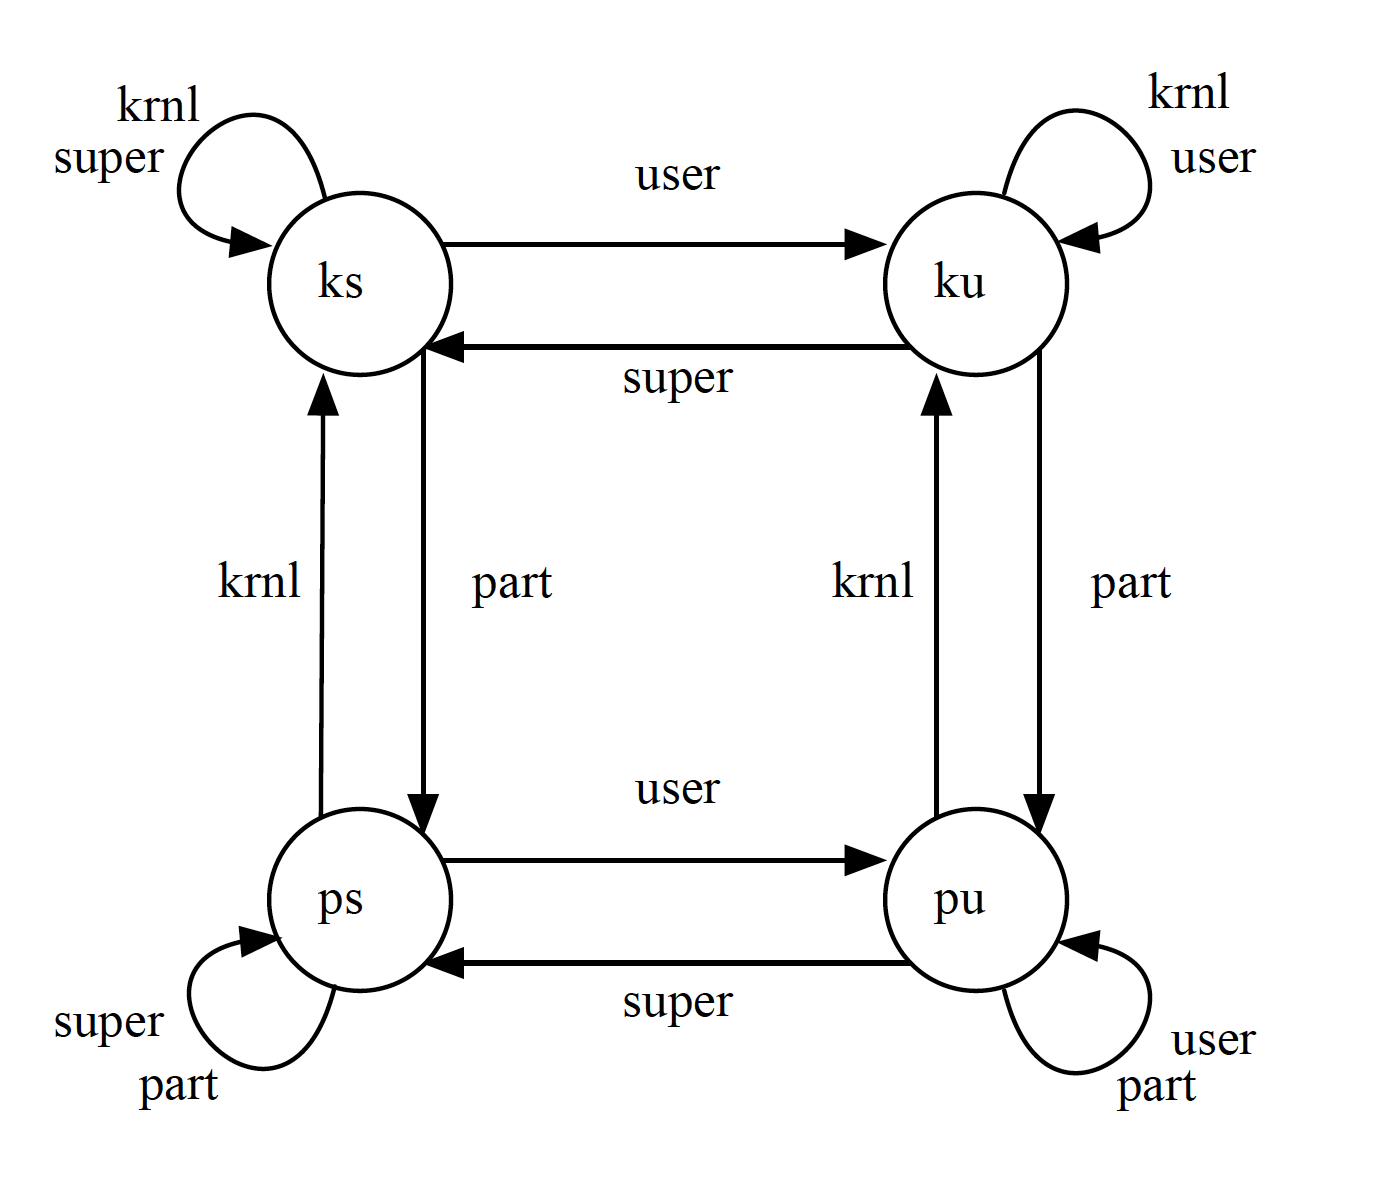
\includegraphics[scale=0.35]{images/CodeModelLTS}

We model the PK-230 requirement by adding a special event that PK-230
will use to signal it has detected a violation:
\begin{circus}
\circchannel scream
\end{circus}
The single step PK-230 check process watches operations,
checking them against who is running, and objects if it sees
partition code executing in supervisor mode:
\begin{circus}
PK230Step \defs \\
\t1 who=KNL \circguard do?i?op \then \Skip \\
\t1 pm=USR \circguard do?i?op \then \Skip \\
\t1 who=PRT \land pm=SUP \circguard scream \then STOP
\end{circus}
It objects by $scream$ing, and then behaving like $\Stop$,
the canonical \Circus/CSP process that always deadlocks.
This also leads to a labelled transistion system,
similar to the above, it with one crucial difference.
Should you enter state $ps$ (partioning,supervisor),
then the only remaining step is to declare a PK-230 violation and deadlock:

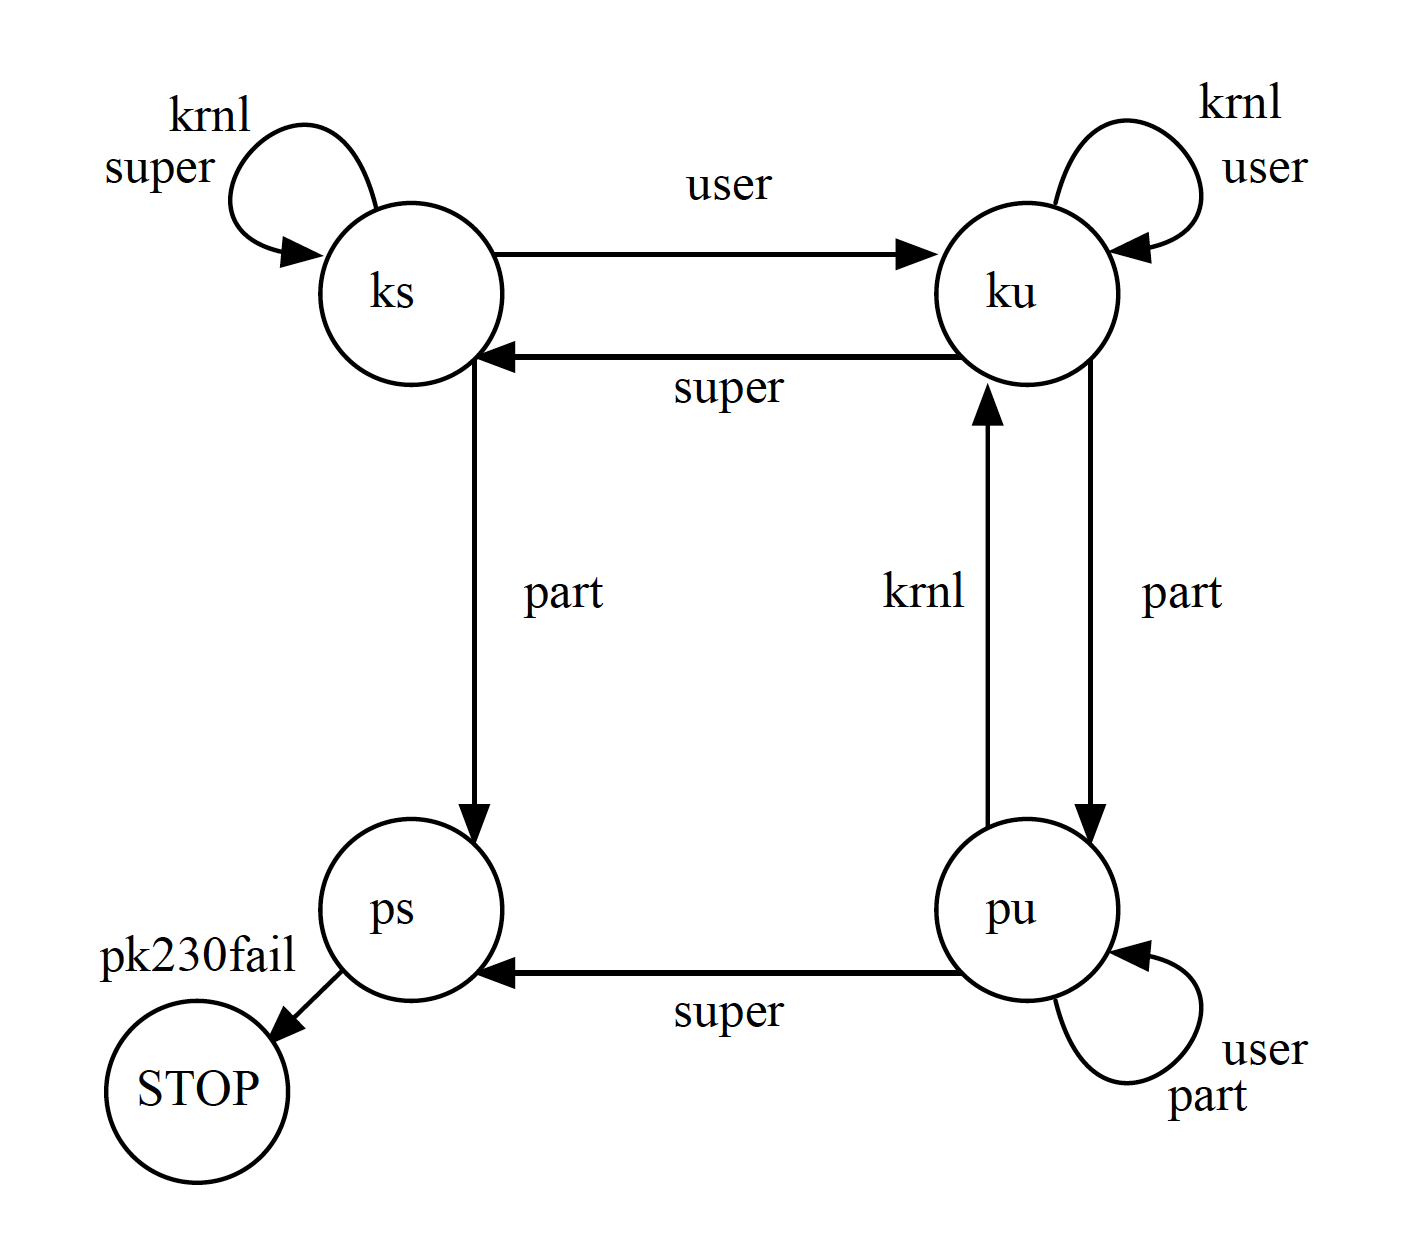
\includegraphics[scale=0.35]{images/PK230LTS}

Normally, we would now model the relevant parts of both kernel and
partition code, but for now lets assume anything can happen,
which is easy---we don't model any code, and just put the platform
in parallel with the requirement.
\begin{circus}
RUN \defs (PMMStep \interleave PK230Step)~; RUN\\
PMMInit \defs pm,who := SUP,KNL \\
PMMInit~; RUN
\end{circus}
This has the effect of modelling
all the possible platform behaviours that might result from any
possible code, correct or otherwise.

The resulting \Circus\ model can then be translated to CSP.
This way we get to see the requirement catching the system out
as shown in Fig. \ref{fig:pk230-scream}.
\begin{figure*}
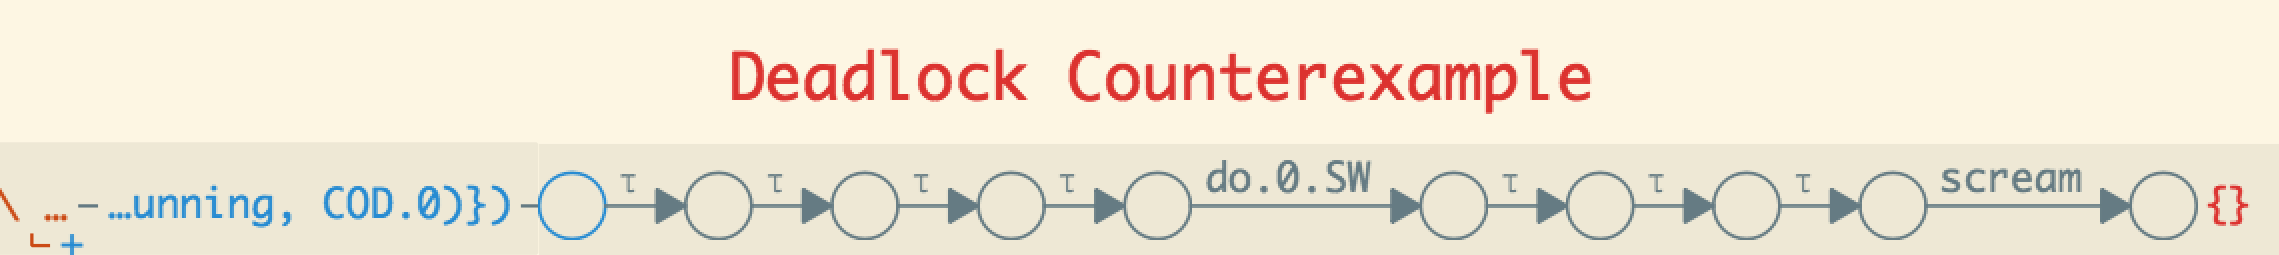
\includegraphics[scale=0.4]{images/PK230-deadlock-example}
\caption{PK-230 objects to partition in SUP mode.}
\label{fig:pk230-scream}
\end{figure*}
Here the kernel, running in supervisor mode, switches to partition
code without changing the mode.

\section{Tool Qualification}

We developed our translation tool to mitigate the difficulty
and risk of error in doing a translation by hand.
However it is legitimate to be concerned about how error-free
our tool is.
Have we faithfully captured the translation as defined in D24.1?
Have our (highly performant) optimisations introdued any futher errors?

Ongoing work is looking at a variety of ways to show that two answers
to the above questions are ``yes'' and ``no'' respectively.
One is the use of FDR itself to compare models,
produced with varying degrees of optimisation,
to each other.
This supplies some good corroboration that we are on the right track.

In addition, there has been considerable work done by colleagues at
the University of York using the Isabelle/HOL theorem prover\cite{NPW02}
to encode the Unifying Theories of Programming (UTP) framework (\textsf{isabelle-utp}),
which is used as the basis for a formal semantics of \Circus,
and to build a series of useful proof automation techniques\cite{FosterZW14}.

We are currently exploring two techniques to use the \textsf{isabelle-utp} framework
to help in verifying the correctness of the translation.
One involves using a tool called Haskabelle \cite{haskabelle09}
that can translate Haskell code into an encoding in Isabelle/HOL
of its formal semantics.
In conjunction with the semantics for \Circus\ and CSP in \textsf{isabelle-utp},
we should then be able to posit and prove the required theorems regarding
translation correctness.
The second is that we can also add a facility to our tool to export both
its \Circus\ input and CSP output to the \textsf{isabelle-utp} notation,
so the correctness of a particular translation instance can be proven.




\section{Conclusion}

We are conducting an on-going investigation into how to formalise
the separation kernel requirements in \cite{IMAKQP-D02},
with an ultimate view to providing a basis for the formal verification
of selected parts of kernel sources w.r.t. those requirements that
may be difficult to test adequately.
Using the \Circus\ notation we are exploring modelling approaches
such as those described above
to assess them in terms of clarity, ease of model-checking, proof support,
and their utility in sderiving formal specifications of code behaviour.
We have also developed tool support to facilitate the analysis
of our \Circus-based models
with existing tools that support CSP.
